\documentclass[14pt]{extbook}
\usepackage{multicol, enumerate, enumitem, hyperref, color, soul, setspace, parskip, fancyhdr} %General Packages
\usepackage{amssymb, amsthm, amsmath, latexsym, units, mathtools} %Math Packages
\everymath{\displaystyle} %All math in Display Style
% Packages with additional options
\usepackage[headsep=0.5cm,headheight=12pt, left=1 in,right= 1 in,top= 1 in,bottom= 1 in]{geometry}
\usepackage[usenames,dvipsnames]{xcolor}
\usepackage{dashrule}  % Package to use the command below to create lines between items
\newcommand{\litem}[1]{\item#1\hspace*{-1cm}\rule{\textwidth}{0.4pt}}
\pagestyle{fancy}
\lhead{Progress Quiz 7}
\chead{}
\rhead{Version B}
\lfoot{6523-2736}
\cfoot{}
\rfoot{test}
\begin{document}

\begin{enumerate}
\litem{
Find the equation of the line described below. Write the linear equation as $ y=mx+b $ and choose the intervals that contain $m$ and $b$.\[ \text{Parallel to } 8 x - 9 y = 8 \text{ and passing through the point } (-5, 6). \]\begin{enumerate}[label=\Alph*.]
\item \( m \in [-1.08, -0.8] \hspace*{3mm} b \in [1.42, 1.58] \)
\item \( m \in [0.47, 1.01] \hspace*{3mm} b \in [10.21, 10.85] \)
\item \( m \in [1.06, 1.31] \hspace*{3mm} b \in [10.21, 10.85] \)
\item \( m \in [0.47, 1.01] \hspace*{3mm} b \in [-10.61, -9.48] \)
\item \( m \in [0.47, 1.01] \hspace*{3mm} b \in [10.55, 11.97] \)

\end{enumerate} }
\litem{
First, find the equation of the line containing the two points below. Then, write the equation as $ y=mx+b $ and choose the intervals that contain $m$ and $b$.\[ (-3, 7) \text{ and } (5, -2) \]\begin{enumerate}[label=\Alph*.]
\item \( m \in [-3.12, 0.88] \hspace*{3mm} b \in [-4.06, -2.99] \)
\item \( m \in [-3.12, 0.88] \hspace*{3mm} b \in [1.14, 4.53] \)
\item \( m \in [-3.12, 0.88] \hspace*{3mm} b \in [-7.14, -6.92] \)
\item \( m \in [1.12, 10.12] \hspace*{3mm} b \in [-8.17, -7.5] \)
\item \( m \in [-3.12, 0.88] \hspace*{3mm} b \in [8.1, 10.9] \)

\end{enumerate} }
\litem{
Solve the equation below. Then, choose the interval that contains the solution.\[ -11(17x -14) = -16(-10x + 18) \]\begin{enumerate}[label=\Alph*.]
\item \( x \in [1.16, 1.96] \)
\item \( x \in [-1.06, -0.24] \)
\item \( x \in [0.31, 0.74] \)
\item \( x \in [-5.79, -4.11] \)
\item \( \text{There are no real solutions.} \)

\end{enumerate} }
\litem{
Solve the linear equation below. Then, choose the interval that contains the solution.\[ \frac{9x + 8}{8} - \frac{-7x + 4}{5} = \frac{8x -5}{3} \]\begin{enumerate}[label=\Alph*.]
\item \( x \in [61.53, 66.53] \)
\item \( x \in [22.47, 29.47] \)
\item \( x \in [-1.23, 2.77] \)
\item \( x \in [10.18, 15.18] \)
\item \( \text{There are no real solutions.} \)

\end{enumerate} }
\litem{
Write the equation of the line in the graph below in Standard form $Ax+By=C$. Then, choose the intervals that contain $A, B, \text{ and } C$.
\begin{center}
    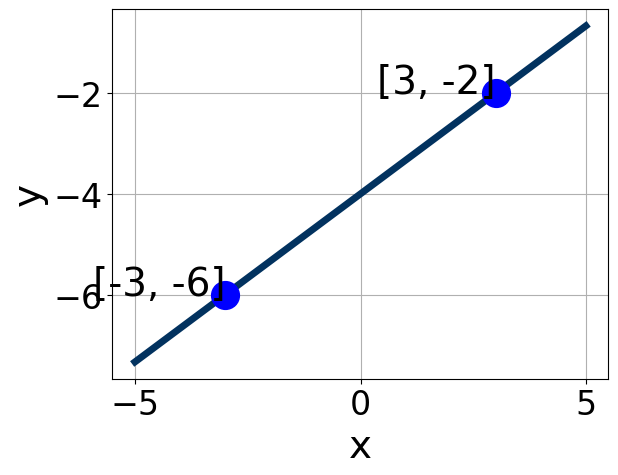
\includegraphics[width=0.5\textwidth]{../Figures/linearGraphToStandardCopyB.png}
\end{center}
\begin{enumerate}[label=\Alph*.]
\item \( A \in [-0.63, 0.45], \hspace{3mm} B \in [-2, 0], \text{ and } \hspace{3mm} C \in [-1, 4] \)
\item \( A \in [-0.63, 0.45], \hspace{3mm} B \in [0, 3], \text{ and } \hspace{3mm} C \in [-1, 4] \)
\item \( A \in [-2.04, -1.08], \hspace{3mm} B \in [5, 6], \text{ and } \hspace{3mm} C \in [-1, 4] \)
\item \( A \in [1.94, 2.47], \hspace{3mm} B \in [5, 6], \text{ and } \hspace{3mm} C \in [-1, 4] \)
\item \( A \in [1.94, 2.47], \hspace{3mm} B \in [-5, -2], \text{ and } \hspace{3mm} C \in [-1, 4] \)

\end{enumerate} }
\litem{
Solve the linear equation below. Then, choose the interval that contains the solution.\[ \frac{-6x -5}{8} - \frac{-7x -9}{2} = \frac{7x -3}{7} \]\begin{enumerate}[label=\Alph*.]
\item \( x \in [0.4, 1] \)
\item \( x \in [-4.6, -3.9] \)
\item \( x \in [-3, -2.2] \)
\item \( x \in [1.8, 4.8] \)
\item \( \text{There are no real solutions.} \)

\end{enumerate} }
\litem{
First, find the equation of the line containing the two points below. Then, write the equation as $ y=mx+b $ and choose the intervals that contain $m$ and $b$.\[ (8, 7) \text{ and } (6, 6) \]\begin{enumerate}[label=\Alph*.]
\item \( m \in [0.36, 1.01] \hspace*{3mm} b \in [-0.69, 0.38] \)
\item \( m \in [-1.09, 0.46] \hspace*{3mm} b \in [7.89, 10.51] \)
\item \( m \in [0.36, 1.01] \hspace*{3mm} b \in [-4.21, -2.47] \)
\item \( m \in [0.36, 1.01] \hspace*{3mm} b \in [-1.59, -0.63] \)
\item \( m \in [0.36, 1.01] \hspace*{3mm} b \in [2.51, 3.47] \)

\end{enumerate} }
\litem{
Solve the equation below. Then, choose the interval that contains the solution.\[ -19(14x -12) = -5(15x -3) \]\begin{enumerate}[label=\Alph*.]
\item \( x \in [0.62, 0.72] \)
\item \( x \in [1.11, 1.15] \)
\item \( x \in [-1.31, -1.25] \)
\item \( x \in [1.21, 1.32] \)
\item \( \text{There are no real solutions.} \)

\end{enumerate} }
\litem{
Write the equation of the line in the graph below in Standard form $Ax+By=C$. Then, choose the intervals that contain $A, B, \text{ and } C$.
\begin{center}
    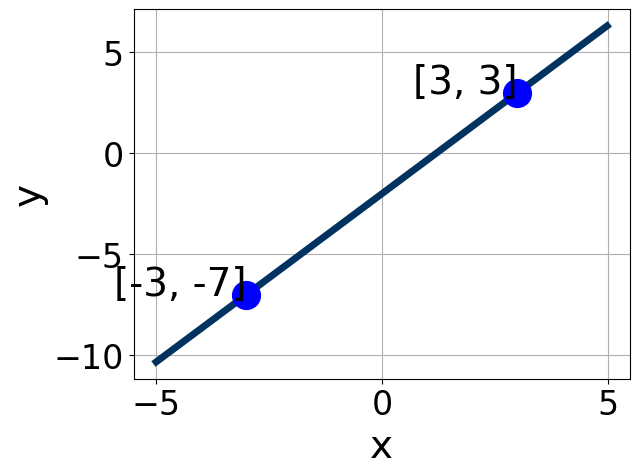
\includegraphics[width=0.5\textwidth]{../Figures/linearGraphToStandardB.png}
\end{center}
\begin{enumerate}[label=\Alph*.]
\item \( A \in [2, 7], \hspace{3mm} B \in [-6.4, -4.6], \text{ and } \hspace{3mm} C \in [10, 12] \)
\item \( A \in [0.5, 1.2], \hspace{3mm} B \in [-1.6, -0.1], \text{ and } \hspace{3mm} C \in [1, 3] \)
\item \( A \in [2, 7], \hspace{3mm} B \in [4, 6.1], \text{ and } \hspace{3mm} C \in [-15, -8] \)
\item \( A \in [-4.7, -1.9], \hspace{3mm} B \in [-6.4, -4.6], \text{ and } \hspace{3mm} C \in [10, 12] \)
\item \( A \in [0.5, 1.2], \hspace{3mm} B \in [-0.1, 1.5], \text{ and } \hspace{3mm} C \in [-4, 1] \)

\end{enumerate} }
\litem{
Find the equation of the line described below. Write the linear equation as $ y=mx+b $ and choose the intervals that contain $m$ and $b$.\[ \text{Parallel to } 9 x - 7 y = 14 \text{ and passing through the point } (-10, 4). \]\begin{enumerate}[label=\Alph*.]
\item \( m \in [-1.73, -0.47] \hspace*{3mm} b \in [-11.86, -3.86] \)
\item \( m \in [0.82, 2.88] \hspace*{3mm} b \in [-16.86, -14.86] \)
\item \( m \in [-0.37, 1.14] \hspace*{3mm} b \in [14.86, 22.86] \)
\item \( m \in [0.82, 2.88] \hspace*{3mm} b \in [14, 15] \)
\item \( m \in [0.82, 2.88] \hspace*{3mm} b \in [14.86, 22.86] \)

\end{enumerate} }
\end{enumerate}

\end{document}